% architecture-diagram.tex — layered block diagram template (standalone).
% Compile: pdflatex/lualatex/xelatex. Output: cropped vector PDF.
\documentclass[tikz,border=4pt]{standalone}
\usetikzlibrary{positioning,arrows.meta}

% ---- one style block; edit here, not per-node -----------------------------
\tikzset{
  block/.style={
    draw, rounded corners=2pt, align=center,
    minimum width=2.6cm, minimum height=0.9cm, font=\small,
  },
  encoder/.style={block, fill=blue!8},
  head/.style={block, fill=orange!12},
  loss/.style={block, fill=green!10},
  data/.style={block, fill=gray!10},
  flow/.style={-{Stealth[length=2.5mm]}, thick},
  skip/.style={flow, dashed, gray},
  stage/.style={font=\footnotesize\itshape, text=gray},
}

\begin{document}
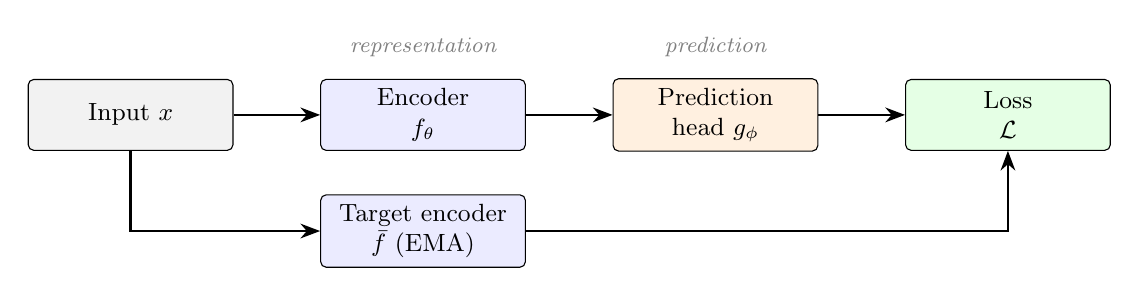
\begin{tikzpicture}[node distance=0.55cm and 1.1cm]

% ---- main chain (positioning, not absolute coords) ------------------------
\node[data]    (input)  {Input $x$};
\node[encoder, right=of input]  (enc)   {Encoder\\$f_\theta$};
\node[head,    right=of enc]    (head)  {Prediction\\head $g_\phi$};
\node[loss,    right=of head]   (loss)  {Loss\\$\mathcal{L}$};

\draw[flow] (input) -- (enc);
\draw[flow] (enc)   -- (head);
\draw[flow] (head)  -- (loss);

% ---- side branch ----------------------------------------------------------
\node[encoder, below=of enc] (target) {Target encoder\\$\bar{f}$ (EMA)};
\draw[flow] (input.south) |- (target.west);
\draw[flow] (target.east) -| (loss.south);

% ---- stage labels ----------------------------------------------------------
\node[stage, above=0.15cm of enc]  {representation};
\node[stage, above=0.15cm of head] {prediction};

\end{tikzpicture}
\end{document}
